\documentclass[a4paper,12pt]{article} % добавить leqno в [] для нумерации слева
\usepackage[a4paper,top=1.3cm,bottom=2cm,left=1.5cm,right=1.5cm,marginparwidth=0.75cm]{geometry}
%%% Работа с русским языком
\usepackage{cmap}					% поиск в PDF
\usepackage{mathtext} 				% русские буквы в фомулах
\usepackage[T2A]{fontenc}			% кодировка
\usepackage[utf8]{inputenc}			% кодировка исходного текста
\usepackage[english,russian]{babel}	% локализация и переносы
\usepackage{multirow}

\usepackage{graphicx}

\usepackage{wrapfig}
\usepackage{tabularx}

\usepackage{hyperref}
\usepackage[rgb]{xcolor}
\hypersetup{
colorlinks=true,urlcolor=blue
}

%%% Дополнительная работа с математикой
\usepackage{amsmath,amsfonts,amssymb,amsthm,mathtools} % AMS
\usepackage{icomma} % "Умная" запятая: $0,2$ --- число, $0, 2$ --- перечисление

%% Номера формул
\mathtoolsset{showonlyrefs=true} % Показывать номера только у тех формул, на которые есть \eqref{} в тексте.

%% Шрифты
\usepackage{euscript}	 % Шрифт Евклид
\usepackage{mathrsfs} % Красивый матшрифт

%% Свои команды
\DeclareMathOperator{\sgn}{\mathop{sgn}}

%% Перенос знаков в формулах (по Львовскому)
\newcommand*{\hm}[1]{#1\nobreak\discretionary{}
{\hbox{$\mathsurround=0pt #1$}}{}}

%% Графики
\usepackage{tikz}
\usepackage{pgfplots}
\pgfplotsset{compat=1.9}

\date{\today}

\begin{document}

\begin{titlepage}
	\begin{center}
		{\large МОСКОВСКИЙ ФИЗИКО-ТЕХНИЧЕСКИЙ ИНСТИТУТ (НАЦИОНАЛЬНЫЙ ИССЛЕДОВАТЕЛЬСКИЙ УНИВЕРСИТЕТ)}
	\end{center}
	\begin{center}
		{\large Физтех-школа аэрокосмических технологий}
	\end{center}
	
	
	\vspace{4.5cm}
	{\huge
		\begin{center}
			{\bf Отчёт о выполнении лабораторной работы 1.2.2}\\
			Экспериментальная проверка закона вращательного движения на крестообразном маятнике
		\end{center}
	}
	\vspace{1cm}
	\begin{center}
		{\large Соболевский Фёдор Александрович \\
			\vspace{0.2cm}
			Б03-109}
	\end{center}
	\vspace{8cm}
	\begin{center}
		Октябрь 2021
	\end{center}
\end{titlepage}

\section{Аннотация}

В данной работе исследован крестообразный маятник и его вращательное движение при приложении к нему постоянного момента сил тяжести. Экспериментально получена зависимость углового ускорения от момента прикладываемых сил и момента инерции вращательной системы. Определён момент инерции маятника. Проанализировано влияние сил трения, действующих на ось вращения, на движение системы.

\section{Теоретические сведения и экспериментальная установка}

В данной работе экспериментально проверяется уравнение вращательного движения:

\begin{equation}
    I\Ddot{\varphi} = M.
    \label{rotationEquation}
\end{equation}

Здесь $ \Ddot{\varphi} \equiv \Dot{\omega} \equiv \beta $ - угловое ускорение системы, $ I $ — полный
момент инерции тела относительно оси вращения, $ M $ — суммарный
момент внешних сил относительной этой оси. Для экспериментального исследования закона вращательного движения (1) в работе использован крестообразный маятник, схематично изображённый на рисунке \ref{setup}. 

\begin{figure}[h]
    \centering
    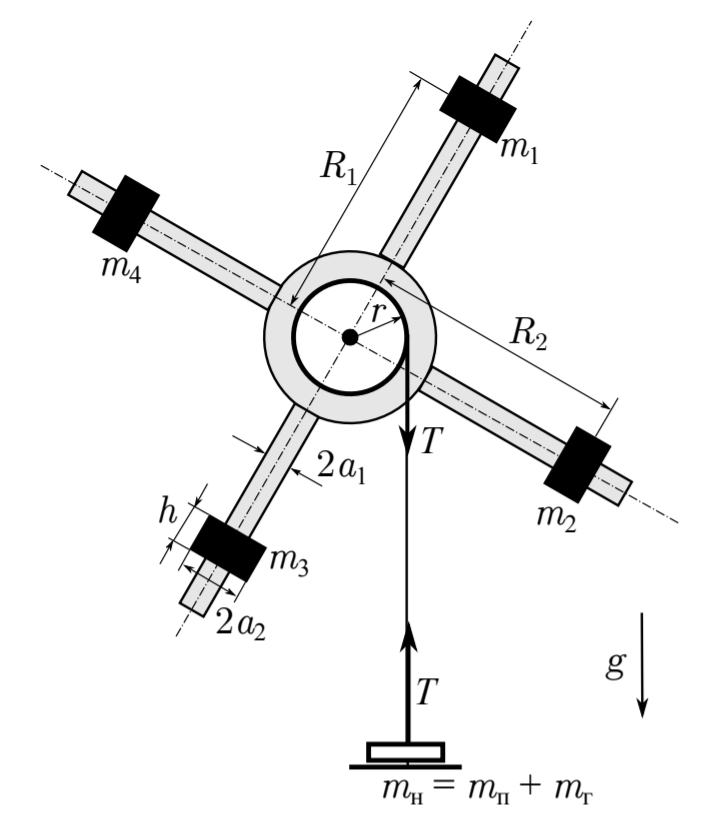
\includegraphics[width = 0.6\textwidth]{1.2.2 setup.PNG}
    \caption{Устройство крестообразного маятника}
    \label{setup}
\end{figure}

Маятник состоит из четырёх тонких стержней радиуса a, закреплённых на втулке под прямым углом друг к другу. Втулка и шкив насажены на общую ось. Ось закреплена в игольчатых подшипниках, так что вся система может свободно вращаться вокруг горизонтальной оси. Передвигая грузы $ m_1 \dots m_4 $ вдоль стержней, можно менять момент инерции маятника. На шкив намотана тонкая нить, к которой привязана лёгкая платформа массы $ m_\text{п} $, служащая для размещения перегрузков $ m_\text{г} $. Установка также оснащена датчиком, фиксирующим моменты времени прохождения концов стержней через него. Данные с датчика передаются на компьютер для последующей обработки и получения значения углового значения, а также зависимостей $ \varphi $ и его производных от времени.

Основной вращающий момент создаётся подвешенным на нити перегрузком вместе с платформой. Непосредственно на маятник действует момент силы натяжения нити $ M = rT $, где $ r $ - радиус шкива. Силу $ T $ можно найти из второго закона Ньютона для платформы с перегрузком: 

\begin{equation}
    m\Ddot{y} = mg - T,
\end{equation}

где $ m = m_\text{п} + m_\text{г} $ - масса платформы с перегрузком. Ускорение платформы связано с угловым ускорением маятника соотношением $ \Ddot{y} = \beta r $. Отсюда момент силы натяжения нити

\begin{equation}
    M = mr(g - \beta r).
    \label{stringMoment}
\end{equation}

К оси вращения также приложен некоторый момент силы трения $ M_\text{тр} $. Таким образом, с учётом \eqref{stringMoment} уравнение \eqref{rotationEquation} приобретает вид

\begin{equation}
    (I + mr^2)\beta = mgr - M_\text{тр}.
\end{equation}

В проведённых опытах $ mr^2 \ll I $, поэтому можно считать, что маятник раскручивается с постоянным угловым ускорением 

\begin{equation}
    \beta_0 = \frac{1}{I}mgr - \frac{M_\text{тр}}{I}
    \label{mainEq}
\end{equation}

Момент инерции системы $ I $ вычисляется с помощью теоремы Гюйгенса-Штейнера (грузы имеют форму полых цилиндров с внутренним и внешним радиусами $ a_1 $ и $ a_2 $ соответственно и образующей $ h $):

\begin{equation}
    I = I_0 + \sum\limits_{i = 1}^4{(\dfrac{1}{12}m_ih^2 + \dfrac{1}{4}m_i(a_1^2 + a_2^2) + m_iR_i^2)}.
    \label{inertiaMoment}
\end{equation}

\section{Оборудование и инструментальные погрешности}

\textbf{Оборудование:} крестообразный маятник, набор перегрузков, платформа для перегрузков, компьютер с измерительной программой, штангенциркуль, весы.

\textbf{Инструментальные погрешности:}

\begin{itemize}
    \item \textbf{Штангенциркуль:} $ \Delta_l^\text{сист} = 0,1 $ мм;
    \item \textbf{Весы:} $ \Delta_m^\text{сист} = 0,1 $ г;
\end{itemize}

Погрешность вычисления программой углового ускорения вычисляется и автоматически выводится вместе с измеренным значением.

\section{Результаты измерений и обработка экспериментальных данных}

\subsection{Оценка момента силы трения в подшипниках}

Для оценки момента силы трения в подшипниках проверялось наличие движения в системе при отсутствии перегрузков на платформе, т.е. когда момент силы натяжения нити создавался исключительно платформой. Массы платформы оказалось достаточно, чтобы привести систему в движение, значит, момент силы трения мал ($ M_\text{тр} < m_\text{п}gr $) и его следует оценивать другим методом.

\subsection{Измерение углового ускорения и момента силы трения}

Измерения углового ускорения проводились для трёх разных положений $ R $ грузов на маятнике при $n=5$ различных значениях массы перегрузков. Радиус шкива $ r = 17,5 $ мм, масса подвеса $ m_\text{п} = 25,4 $ г.  Результаты измерений представлены в таблицах 

\begin{table}[h]
    \centering
    \begin{tabular}{|c|c|c|c|c|c|c|c|c|} \hline
         \multicolumn{3}{|c|}{ } & \multicolumn{2}{c|}{$R = 50$ мм} & \multicolumn{2}{c|}{$R = 100$ мм} & \multicolumn{2}{c|}{$R = 150$ мм} \\ \hline
        № & $m_\text{г}$ , г & $ M $, $ 10^{-4} $ Н $\cdot$ м & $\beta$, рад/$ \text{с}^2 $ & $\sigma_\beta$, рад/$ \text{с}^2 $ & $\beta$ & $\sigma_\beta$ & $\beta$ & $\sigma_\beta$ \\ \hline
        1 & 27,1 & 90,13 & 1,117 & 0,012 & 0,674 & 0,004 & 0,4206 & 0,0017 \\ \hline
        2 & 44,6 & 120,17 & 1,552 & 0,010 & 0,928 & 0,003 & 0,5590 & 0,0024 \\ \hline
        3 & 62,9 & 151,59 & 2,007 & 0,008 & 1,165 & 0,006 & 0,727 & 0,003 \\ \hline
        4 & 74,1 & 170,82 & 2,247 & 0,004 & 1,351 & 0,004 & 0,8234 & 0,0015 \\ \hline
        5 & 101,2 & 217,34 & 2,901 & 0,010 & 1,743 & 0,005 & 1,0730 & 0,0021 \\ \hline 
    \end{tabular}
    \caption{Значения углового ускорения при разных параметрах системы}
    \label{tab:res1}
\end{table}

По результатам измерений можно построить график зависимости $ \beta $ от $ M $: $ \beta = kM - b $, где $ k = \frac{1}{I} $, $ b = \frac{M_\text{тр}}{I} $ (из уравнения \eqref{mainEq}). Коэффициенты $ k $ и $ b $ и погрешности их вычисления определим методом наименьших квадратов:

\begin{equation}
    k = \frac{\langle \beta M \rangle - \langle \beta \rangle \langle M \rangle}{\langle M^2 \rangle - \langle M \rangle^2} 
\end{equation}

\begin{equation}
    -b = \langle \beta \rangle - k \langle M \rangle ;
\end{equation}

\begin{equation}
    \sigma_k = \frac{1}{\sqrt{n}} \sqrt{\frac{\langle \beta^2 \rangle - \langle \beta \rangle^2}{\langle M^2 \rangle - \langle M \rangle^2} - k^2},
\end{equation}

\begin{equation}
    \sigma_b = \sigma_k \sqrt{\langle M^2 \rangle - \langle M \rangle^2}.
\end{equation}

Отсюда можно найти значения момента инерции установки $ I $ и момента силы трения $ M_\text{тр} $ и их погрешности:

\begin{equation}
    I = \frac{1}{k}, \text{    } \sigma_I = I \frac{\sigma_k}{k};
\end{equation}

\begin{equation}
    M_\text{тр} = Ib, \text{    } \sigma_{M_\text{тр}} = M_\text{тр} \sqrt{(\frac{\sigma_b}{b})^2 + (\frac{\sigma_I}{I})^2};
\end{equation}

\begin{table}[h]
    \centering
    \begin{tabular}{|c|c|c|c|c|c|c|c|c|} \hline
        $ R $, мм & $ k $, $ \frac{1}{\text{кг} \cdot \text{м}^2} $ & $ \sigma_k $, $ \frac{1}{\text{кг} \cdot \text{м}^2} $ & $ b $, $ \frac{\text{Н}}{\text{кг} \cdot \text{м}} $ & $\sigma_b $, $ \frac{\text{Н}}{\text{кг} \cdot \text{м}} $ & $ I $, $ \text{кг} \cdot \text{м}^2 $ & $ \sigma_I $, $ \text{кг} \cdot \text{м}^2 $ & $ M_\text{тр} $, Н $ \cdot $ м & $ \sigma_{M_\text{тр}} $, Н $ \cdot $ м \\ [5pt]\hline
        50 & 139,8 & 1,2 & 0,132 & 0,005 & 0,00715 & 0,00006 & 0,00094 & 0,00004 \\ \hline
        100 & 83,9 & 1,1 & 0,087 & 0,005 & 0,01192 & 0,00015 & 0,00103 & 0,00006 \\ \hline
        150 & 51,5 & 0,6 & 0,0523 & 0,0027 & 0,01941 & 0,00024 & 0,00101 & 0,00006 \\ \hline
    \end{tabular}
    \caption{Значения коэффициентов наилучших прямых, моментов инерции и момента силы трения}
    \label{tab:res2}
\end{table}

Полученные значения  представлены в таблице \ref{tab:res2}. Графики зависимости $ \beta $ от $ M $ изображены на рисунке \ref{graph}.

\begin{figure}
\centering
\resizebox {0.7\textwidth} {!} {
\begin{tikzpicture}
\begin{axis}[ xlabel = {$ M $, $ 10^{-4} $ Н $\cdot$ м}, ylabel = {$ \beta $, рад/$ \text{с}^2 $}, xmin = 0, xmax = 235, ymin = 0, ymax = 3, legend style={legend style={at={(axis cs:5, 2.05)},anchor=south west}}]

\addplot[color=black, mark=x, only marks] coordinates{(90.13, 1.117)(120.17, 1.552)(151.59, 2.007)(170.82, 2.247)(217.34, 2.901)};
\addplot[color=black, mark=o, only marks] coordinates{(90.13, 0.674)(120.17, 0.928)(151.59, 1.165)(170.82, 1.351)(217.34, 1.743)};
\addplot[color=black, mark=triangle, only marks] coordinates{(90.13, 0.4206)(120.17, 0.559)(151.59, 0.727)(170.82, 0.8234)(217.34, 1.073)};

\legend{$ R = 50 $ мм, $ R = 100 $ мм, $ R = 150 $ мм}

\addplot[color=blue] coordinates{(9.4, 0)(217.34, 2.901)};
\addplot[color=red] coordinates{(10.3, 0)(217.34, 1.743)};
\addplot[color=blue] coordinates{(10.1, 0)(217.34, 1.073)};

\end{axis}
\end{tikzpicture}
}
\caption{Зависимость углового ускорения маятника от момента сил тяжести}
\label{graph}
\end{figure}

\subsection{Измерение момента инерции маятника}

По вычисленному в пункте 4.2 значению момента инерции системы $ I $ при различных $ R $ можем найти момент инерции маятника без грузов. Для этого можно использовать формулу \eqref{inertiaMoment}. 

Параметры маятника:

\begin{itemize}
    \item $ m_1 = 151,7 $ г;
    \item $ m_2 = 158,2 $ г;
    \item $ m_3 = 152,6 $ г;
    \item $ m_4 = 157,0 $ г;
    \item $ R_1 \approx ... \approx R_4 $;
    \item $ h = 25 $ мм;
    \item $ a_1 = 3,8 $ мм;
    \item $ a_2 = 17,5 $ мм;
\end{itemize} 

Выразим из формулы \eqref{inertiaMoment} момент инерции $ I_0 $:

\begin{equation}
    I_0 = I - \sum\limits_{i = 1}^4{(\dfrac{1}{12}m_ih^2 + \dfrac{1}{4}m_i(a_1^2 + a_2^2) + m_iR_i^2)}
\end{equation}

Погрешность вычисления $ I_0 $ по данной формуле

\begin{equation}
    \sigma_{I_0} = \sqrt{\sigma_I^2 + (I - I_0)^2((\frac{2\Delta_m^\text{сист}}{\sum m_i})^2 + (\frac{\frac{19}{6}\Delta_l^\text{сист}}{\frac{1}{12}h^2 + \frac{1}{4}(a_1^2 + a_2^2) + R^2})^2)}
\end{equation}

\begin{table}[]
    \centering
    \begin{tabular}{|c|c|c|c|} \hline
        $ R $, мм & 50 & 100 & 150 \\ \hline
        $ I $, $ 10^{-3} \text{кг} \cdot \text{м}^2 $ & 7,15 & 11,92 & 19,41 \\ \hline
        $ I_0 $, $ 10^{-3} \text{кг} \cdot \text{м}^2 $ & 5,52 & 5,64 & 5,39 \\ \hline
        $ \sigma_{I_0} $, $ 10^{-3} \text{кг} \cdot \text{м}^2 $ & 0,20 & 0,21 & 0,21 \\ \hline
    \end{tabular}
    \caption{Результаты вычисления собственного момента инерции маятника}
    \label{tab:aboba}
\end{table}

В таблице \ref{tab:aboba} представлены найденные при разных $ R $ значения момента инерции маятника $ I_0 $. Они не отличаются друг от друга больше, чем на $ \approx \sigma_{I_0} $. Для проверки применимости формулы \eqref{inertiaMoment} было измерено угловое ускорение маятника без грузов при $ m_\text{г} = 27,1 $ г: $ \beta = 1,63 $ рад/$ \text{с}^2 $, откуда из \eqref{mainEq} $ I_0 = \frac{M - M_\text{тр}}{\beta} \approx 5,3 \cdot 10^{-3} \text{кг} \cdot \text{м}^2 $. Это значение близко к вычисленным по формуле \eqref{inertiaMoment}, поэтому её можно считать применимой.

\section{Обсуждение результатов и вывод}

Полученные в ходе работы экспериментальные и теоретические значения собственного момента инерции маятника приблизительно равны и различаются в пределах погрешности измерений. Для разных моментов инерции маятника вычисленные моменты силы трения в оси оказались приблизительно равными, что соответствует действительности и подтверждает справедливость используемых формул и допустимых приближений. Точности эксперимента достаточно, чтобы проверить все рассмотренные в работе теоретические закономерности, однако для измерения моментов инерции предпочтительнее другие методы, так как ошибка в данном опыте может оказаться слишком большой для более точных измерений.

\begin{equation}\label{lel}
    \Vec{E} = \Vec{E_0}\cos(\omega t - \vec{k}\vec{r} + \varphi_0).
\end{equation}

I have achieved \ref{lel}.

\end{document}